% Harshad Deshmukh (harshad@cs.wisc.edu)
% Ph.D. Thesis

% Using template from Burr Settles:
% Improvements to the LaTeX "withesis" class, made by Burr Settles
% Intended mainly for writing a CS Department PhD thesis.
% Assumes compilation using pdflatex.


% differences between "official" print and online PDF versions:
%  - change documentclass command (below)
%  - uncomment out "singlespace" (below)
%  - comment out separator page that fixes TOC bug (withesis.cls, line 386)
%  - uncomment "hyperref" commands for hyperlinked PDF (below)

%=====================================================================
% Document Style
%=====================================================================

%\documentclass[12pt,twoside]{withesis}      % for online PDF
\documentclass[12pt]{withesis}              % for official version

% packages
\usepackage{times}
\usepackage{amssymb,amsmath}
\usepackage[chapter]{algorithm}
\usepackage{algorithmicx}
\usepackage{algpseudocode}
%\usepackage{algorithmic}
%\usepackage{algorithm2e}
\usepackage{graphicx}   % for includegraphics
\usepackage{color}      % for "to do" command
\usepackage{balance}
\usepackage{natbib}     % preferred bibliography style
\usepackage{makeidx}    % to make the index
\usepackage{rotating}
\usepackage{multirow}
\usepackage{mathtools}  % chrisr added to get symbol for :-
\usepackage{longtable}
\usepackage{url}
\usepackage{epsfig,amsfonts}
\usepackage{amsthm}
\usepackage{enumerate}

%% Chaitanya
\usepackage{pbox}
\usepackage{multirow}
\usepackage{caption}
\usepackage{subcaption}
\DeclareCaptionType{copyrightbox}

\usepackage{pifont}
\usepackage{array}

% "hyperref" package for making section/citation references hyperlinks
% note: run "make clean" if swtiching from hyperref to non-hyperref, and
% vice versa, as they use different TOC file markups.

% \usepackage{hyperref}
% 
% \definecolor{links}{rgb}{0.5,0,0} 
% \definecolor{cites}{rgb}{0,0.5,0} 
% \definecolor{urls}{rgb}{0,0,0.5} 
% 
% \hypersetup{
%     bookmarks=true,         % show bookmarks bar?
%     pdftitle={A PhD Thesis},
%     pdfauthor={Buckingham M. Badger},
%     pdfkeywords={machine learning, badgers, beer},
%     pdfnewwindow=true,      % links in new window
%     colorlinks=true,       % false: boxed links; true: colored links
%     linkcolor=links,          % color of internal links
%     citecolor=cites,        % color of links to bibliography
%     % filecolor=black,      % color of file links
%     urlcolor=urls           % color of extern	al links
% }

% my custom definitions
%\usepackage{mymacros}
%\bibpunct{(}{)}{;}{a}{,}{,} % parens in citations instead of brackets for "natbib" style

\makeindex

%========================================================================
%  Draft Control Commands:
%========================================================================
\pagestyle{thesis}

%========================================================================
% Remove the following lines if appendix tables or figures are present.
% The suppress writing the auxiliary information which appears in the
% list of tables or list of figures.

\noappendixtables                % Don't have appendix tables
\noappendixfigures               % Don't have appendix figures

% End of Preamble, start of document
\begin{document}
% \singlespace                  % toggle single- or double-spaced version

% prelude.tex
%   - titlepage
%   - dedication
%   - acknowledgments
%   - table of contents, list of tables and list of figures
%   - nomenclature
%   - abstract
%============================================================================

\clearpage\pagenumbering{roman}  % This makes the page numbers Roman (i, ii, etc)

% TITLE PAGE
\title{Efficient Query Scheduling}
\author{Harshad Deshmukh}
\date{2018}
\dissertation
\department{Computer Sciences}
\oralexamdate{07/13/2018}
\committeeone{Jignesh Patel, Professor, Computer Sciences, UW-Madison}
\committeetwo{Paraschos Koutris, Assistant Professor, Computer Sciences, UW-Madison}
\committeethree{Andrea Arpaci-Dusseau, Professor, Computer Sciences, UW-Madison}
\committeefour{Theodoros Rekatsinas, Assistant Professor, Computer Sciences, UW-Madison}
\committeefive{Remzi Arpaci-Dusseau, Professor, Computer Sciences, UW-Madison}

\maketitle

% COPYRIGHT PAGE
%   - To include a copyright page use \copyrightpage
\copyrightpage

% DEDICATION
\begin{dedication}
    \emph{To Supriya}
\end{dedication}

% ACKNOWLEDGMENTS
\begin{acknowledgments}
    \singlespace
    This journey has been possible due to so many helping hands in my life. 
First and foremost, my advisor Prof. Jignesh Patel. 
Jignesh's infectious energy and his passion for database research have shaped many ideas in my work.
I find it fascinating that he can dive into low level implementation details with the same ease as he can paint the big picture.
I benefited tremendously by his feedback on my writing and presentation skills. 
He always prioritized my well being and my family's well being over other things. 
I hope to emulate his industriousness, discipline and remarkable interpersonal communication skills. 

I was fortunate to be in Wisconsin's database group and interact with some astounding professors. 
Jeff Naughton during his time in Wisconsin was like a father figure. 
His sharp and witty comments during the talks always made the atmosphere lively. 
I hope to enjoy Jeff's mentorship in my professional life. 
I have had numerous interactions with AnHai Doan.
I am grateful for his advice and support during my job search.
I thank my committee members Professors Paris Koutris, Theodoros Rekatsinas, Andrea Arpaci-Dusseau and Remzi Arpaci-Dusseau for reading my dissertation and for their helpful comments. 

I am grateful to the Computer Sciences Graduate Coordinator Angela Thorp for her support in administrative matters. 

I could live a debt free grad school life, thanks to the grants from the National Science Foundation.
This money essentially comes from the tax dollars of hardworking American men and women.
My sincere thanks to all of them.

Quickstep is a group project and is built from the contributions of several students.
My work would not have been possible without their collective efforts. 
I would like to thank Quickstep developers including Craig Chasseur, Qiang Zeng, Shoban Chandrabose, Yinan Li, Gerald, Zuyu Zhang, Jianqiao Zhu, Rathijit Sen, Saket Saurabh, Navneet Potti, and Udip Pant and Quickstep's Apache mentor Julian Hyde.  

I got a chance to do multiple internships in grad school. 
I am grateful to my Samsung internship colleagues Chang-Ho Choi and Suraj Waghulde for their support. 
I learnt a great deal at my internship with Microsoft CISL.
Avrilia Floratou was a great mentor and I learnt from her the \textit{modus operandi} of industrial research.
Ashvin Agrawal was a great collaborator who taught me a great deal about rapid software prototyping. 
Prajakta Kalmegh and I became good friends through car pool. 
%The really smart and nice people in CISL including Sriram Rao, Carlo Curino, Subramaniam Krishnan, Chris Cai, Konstantinos Karanasos, Chris Douglas, Virajith Jalaparty, and Arun Suresh made the internship a memorable experience. 

Life would have been very difficult without some great friends in the database group. 
Yash Govind has been a great friend and confidant.
Shaleen Deep was the sounding board for a lot of my silly ideas.
Adalbert Gerald Soosai Raj has provided immense support through good times and bad. 
I developed close friendship with Hakan Memisoglu during his time in Wisconsin.
Whenever I needed help, Rogers Jeffrey Leo John would always come along with his (poor?) jokes. 
I learnt a great deal from the long interactions with Bruhathi on the pipelining project, as well as during my job search.
Pradap Konda Venkatraman's mature demeanor and deep insights had a calming effect on me.
I thank Adel Ardalan for his help on my various presentations. 
Paul Suganthan GC helped me find accommodation during my first summer in Wisconsin. 
I had a great time working with Vinitha Reddy on many course projects.

Through the years, I had the company of some wonderful office mates. 
They often accompanied me to Peet's for coffee breaks and helped me refresh from the work.
The long chats with Hakan Memisoglu and Marc Spehlmann made walks to Gordon dining center seem like a breeze.
I am grateful to Spyros Blanas for his tidbits of wisdom. 
An incomplete list of otther officemates include Sriram Sridharan, Yueh-Hsuan Chiang, Lalitha Viswanathan, Han Li, and Dylan Bacon.

I got to know several bright and kind people in the UW over the years. 
Prashant Saxena was my roommate for the first two years and his sense of humour would always lighten up the atmosphere. 
I had several insightful discussions with Prashant over the delicious dinners he cooked. 
I thoroughly relished Ankit Agrawal's company during his Master's.
Ankit and I could talk for hours about anything under the sun.
I still remember Friday evening tea parties with Ankit and Nishant Agrawal. 
Sanketh Nalli remains a good friend till date.
Meenakshi Syamkumar has become a close family friend. 
I am grateful to Ramnatthan Alagappan and Aishwarya Ganesan for their company for dinners and fun outings.
An incomplete list of friends in the UW include Rohit Bhat, Junaid Khalid, Ashutosh Pandey, Swapnil Haria, Amrita Roy Chowdhury, Neha Godwal, Kushagra Garg, and Sakshi Gupta. 

My under-graduation institute BITS Pilani has a special place in my life.
Many friendships from BITS have accompanied me from India to the US. 
I have had many trips in grad school with these friends which helped me refresh.

Soumyadeep Ghosh has been a close friend ever since under-graduation days and till date he's my goto person for venting out frustration. 
I am grateful to Aditya Vijay's great advice in so many situations.
Ankur Gupta provided great company on various trips that we went on together.

My friends from Pilani continue to provide me moments of great joy.
I am greateful to Ameya Zambre, Nilesh Deshpande, Jhinak Sen, Vineet Pandey, Apoorv Bapat, Akash Badave, Aditya Belsare, Aditya Sharma, Ashirvad Singh, Chanchal Batra, Abhishek Jain, Subhro Sarkar, Priyanka Gupta and Pooja Chandra.

%I spent the first two years of my grad school working on the BITS2MSPhD project to provide MS/PhD related assistance to aspiring undergraduates from BITS. 
%Volunteering for BITS2MSPhD while in grad school helped me manage my time better.
%I had a great time working with Varsha Rajshekhar, Yash Gandhi, Manish Kumar, Adwait Gandhe and Ishaan Biswas. 

Living in Madison would be dull without a fantastic group of friends.
I met a lot of people through Maharashtra Mandal in Madison.
Thanks to all of them for the joyful cultural events and parties.
%I am grateful to Kimaya and Rohan Pradhan, Girish and Priti Kulkarni, Nikhil and Tanuja Jog, Abhishek and Nishi Kulkarni, Milind and Rama Ranade, Abhinav and Nishita Verma, Stimit and Vidhi Shah, and Ojas Kale for the numerous parties and fun times together. 

Family is the ultimate support system. 
My in laws Anant and Neha Hirurkar always supported my pursuit of PhD. 
My sisters Sukhada and Sampada and their husbands Akshay and Hitesh encouraged me to follow my aspirations and took great care of my parents.
My nephews and niece provided great joy during my trips to India.

I dearly miss my late maternal grandmother. 
She was a single mother and a primary school teacher.
She raised six kids on a meager income.
Despite the hardships, she had a staunch belief in the power of education.
She has a profound influence on my life.

I can probably never do enough to repay what my parents have done for me. 
They made several sacrifices to ensure that I got a high quality education. 
They always believed in my decisions and supported me in tough times.
Whatever little success that I have achieved is a testimony to their strong foundational values.
Thank you Aai and Baba from the bottom of my heart.

I got the gift of fatherhood during grad school.
Being a father to an adorable little girl felt daunting at time, but ultimately was a very rewarding feeling.
All the stress from working in grad school would go away with a single smile of my daughter.

Last, but by no means the least, I would like to thank my wonderful wife Supriya. 
She always believed in me, even when I doubted myself. 
In bad times or good, she always kept assuring me that I was capable of making it to the finish line. 
She went to such extremes that I was not allowed to crack jokes on myself! 
She sacrificed her professional life and single handedly managed our family life so that I could focus on my PhD. 
Supriya, you made all the hardships worthwhile! 
\end{acknowledgments}

% CONTENTS, TABLES, FIGURES
\tableofcontents
\listoftables
\listoffigures

%\listofalgorithms
%\addcontentsline{toc}{chapter}{List of algorithms}

%=============================================================================
% UMI ABSTRACT
%=============================================================================
% The UMI abstract should begin with the author and title in a standard format.
% After the author comes the advisor and university. After these lines comes
% a bunch of double spaced text to make up the standard abstract.
% After the abstract, the advisor's approval signature follows.
% This page is not numbered and is delivered seperately to the thesis office.
%=============================================================================



%% UMI ABSTRACT
%     \pagestyle{empty}   % Turns off page numbering
    % \addtocounter{page}{-1} % Noto:  Subtract an ADDITIONAL page because my abstract goes two pages.
%     \advisorname{AnHai Doan}
%     \advisortitle{Associate Professor}
%     \begin{umiabstract}
%       Analytical database systems process data to find insights. 
Database systems today are facing challenges from multiple fronts: First, there is an unprecedented data being generated by machines and humans.
Second, there is a diverse demand for analytics which includes relational analytics used for reporting and predictive analytics for forecasting.
Third, the hardware landscape keeps evolving which means the database system need to keep up in order to reap the best out of the hardware.
Finally cloud computing challenges the many assumptions that the traditional systems were built on with regards to deployment environments and availability of computing, storage and network resources.
Given these challenges, the modern database systems need to manage the resources at their disposal \textit{efficiently} - to produce faster results, \textit{effectively} - to fully utilize the resources and \textit{transparently} - to be accountable to its users.

In this dissertation, we present the query scheduler of Quickstep database system that imparts efficiency, effectiveness and transparency to the resource management of Quickstep. 

In the first chapter we present the makeup of the Quickstep system. 
We describe a task abstraction called Work Orders, which are managed by the scheduler.
Through work orders, Quickstep scheduler obtains fine grained control over query execution, and allows the system to exploit large amounts of parallelism offered by modern hardware.

Next we showcase the usefulness of the Quickstep scheduler as it solves two challenges: resource governance and performance.
In the second chapter, we employ the Quickstep scheduler for allocating resources such as CPU to concurrent users of the system.
The resource allocation can understand high level policies such as fair and priority-based, and enforces them while allocating the resources.
The scheduler has a learning component, which constantly monitors the resource consumption happening in the system, anticipates the future resource requirements and adjusts the resource allocation so as to meet the policy goals.
Our experiments demonstrate that we are able to meet the goals as per the policy specifications.

In the final chapter, we highlight the impact of scheduling techniques on individual query performance.
We turn to pipelining, which is a well known query processing technique, used since the times of disk-based systems.
We revisit the importance of pipelining in the in-memory systems and examine the role of various parameters such as block size, parallelism, storage format and hardware prefetching.
For queries with complex query plans, we also provide a pipeline sequencing algorithm so as to efficiently process the pipelines and complete the query execution. 
%     \end{umiabstract}
%     \pagestyle{thesis} % Turns page numbering back on

% REGULAR ABSTRACT
%\begin{abstract}
%    %\singlespace
%    Analytical database systems process data to find insights. 
Database systems today are facing challenges from multiple fronts: First, there is an unprecedented data being generated by machines and humans.
Second, there is a diverse demand for analytics which includes relational analytics used for reporting and predictive analytics for forecasting.
Third, the hardware landscape keeps evolving which means the database system need to keep up in order to reap the best out of the hardware.
Finally cloud computing challenges the many assumptions that the traditional systems were built on with regards to deployment environments and availability of computing, storage and network resources.
Given these challenges, the modern database systems need to manage the resources at their disposal \textit{efficiently} - to produce faster results, \textit{effectively} - to fully utilize the resources and \textit{transparently} - to be accountable to its users.

In this dissertation, we present the query scheduler of Quickstep database system that imparts efficiency, effectiveness and transparency to the resource management of Quickstep. 

In the first chapter we present the makeup of the Quickstep system. 
We describe a task abstraction called Work Orders, which are managed by the scheduler.
Through work orders, Quickstep scheduler obtains fine grained control over query execution, and allows the system to exploit large amounts of parallelism offered by modern hardware.

Next we showcase the usefulness of the Quickstep scheduler as it solves two challenges: resource governance and performance.
In the second chapter, we employ the Quickstep scheduler for allocating resources such as CPU to concurrent users of the system.
The resource allocation can understand high level policies such as fair and priority-based, and enforces them while allocating the resources.
The scheduler has a learning component, which constantly monitors the resource consumption happening in the system, anticipates the future resource requirements and adjusts the resource allocation so as to meet the policy goals.
Our experiments demonstrate that we are able to meet the goals as per the policy specifications.

In the final chapter, we highlight the impact of scheduling techniques on individual query performance.
We turn to pipelining, which is a well known query processing technique, used since the times of disk-based systems.
We revisit the importance of pipelining in the in-memory systems and examine the role of various parameters such as block size, parallelism, storage format and hardware prefetching.
For queries with complex query plans, we also provide a pipeline sequencing algorithm so as to efficiently process the pipelines and complete the query execution. 
%\end{abstract}
% ~\newpage


% NOMENCLATURE
%\begin{nomenclature}
%\input{frontmatter/nomenclature}
%\end{nomenclature}

%\clearpage\pagenumbering{arabic} % This makes the page numbers Arabic (1, 2, etc)
\pagenumbering{arabic} % This makes the page numbers Arabic (1, 2, etc)
   % title page, abstract, contents, etc.

%% Acknowledgements 		   	%% Needs 1 hour 	#2

%=======================================================================
% Chapter tex files
%\include{intro/intro2}
%\include{background/background1}
%\include{synfinder/synfinder1}
%\include{rmony/rmony4}
%\include{falcon/falcon4}
%\include{smurf/smurf1}
%\include{opensource/opensource1}
%\include{discussion/discussion}
%\chapter{Conclusions and Future Work}
In this chapter, we discuss the lessons learnt, present our conclusions, and describe the future work.
Through this dissertation, we present the design and implementation of a query scheduler.
The goal of this scheduler is to efficiently execute queries in an in-memory environment while effectively exploiting the features provided by the modern hardware. 
A key contribution of this dissertation is to demonstrate that the scheduler is capable of playing an important role in the database system architecture.

\section{Lessons Learnt}
We now discuss the lessons learnt from this dissertation.

\subsection{Importance of Abstraction and Contracts}
A good abstraction is vital for developing a good system. 
The work order abstraction in Quickstep proved to be a boon for the query scheduler. 
It allowed us to construct different layers on top of simple operator execution, for which the  abstraction was created. 

There was a clarity of the contract between query optimizer and query scheduler: the query optimizer creates an immutable query plan (DAG of relational operators), which is then passed on to the query scheduler. 
Once the query scheduler starts to operate on the query plan, there is no going back to the optimizer. 

We designed the operators to be stateful and allowed the scheduler to access their state thereby getting more insights about the query execution progress.
The book-keeping related data structures are handled only by the scheduler thread, thus they need not be thread-safe, which helped simplify their design. 

\subsection{Importance of Query Scheduler for High Performance}
Achieving high performance is a never unending pursuit for database systems. 
Though the scheduler has a lot of power in terms of controlling resources and co-ordinating the query execution, it still needs support from other modules in the database system for high performance.
Query optimizer is a vital component of the system. 
Scheduling work for an optimal query plan is far more effective than that for a poor plan. 
Moreover, efficient implementation of relational operators is crucial to leverage the most from the hardware. 
Therefore, even though the scheduler is an important piece in the overall puzzle, it must work in tandem with other components in the system. 

\subsection{Importance of Measurement, Estimation, and Analysis}
Measuring and estimating performance in systems is highly important. 
Back-of-the-envelope calculations is a handy technique that can be useful to anticipate the effect of a technique or a change.
By doing such calculations, we may be able to save a lot of development effort. 

Our work on revisiting pipelining relied heavily on measuring performance and analyzing the impact of various techniques on performance. 
Putting the performance improvement of pipelining into perspective was only possible due to the emphasis on measurement.
We made lot of mistakes in attributing performance changes to wrong reasons and learnt some valuable lessons the hard way.

While dealing with many parameters, it is important to adhere to basic scientific principles, e.g, not changing two parameters simultaneously, while studying the effect of one.

%Between multi-core CPU and memory, which are the primary kinds of resources used by an in-memory database system; CPU is 
\section{Conclusions}
We now discuss the conclusions from individual chapters of this dissertation. 

In Chapter~\ref{chap:quickstep}, we present the design and implementation of the Quickstep database system. 
Quickstep has a unique block based storage management system, that supports variety of storage formats such as row store, column store along with support for compression. 
The query execution in Quickstep happens with the help of a task abstraction called work orders. 
The work orders abstraction connects storage management in Quickstep with the execution engine. 
Quickstep's query scheduler, which is the focus of this dissertation controls the execution of these work orders and thus manages query execution in the system. 
Through our experimental evaluation, we show that the intra-operator and inter-operator parallelism through the work orders abstraction speeds up the query execution in Quickstep.
The work order abstraction is instrumental for realizing intra-operator parallellism.
Comparison with other systems also show that Quickstep is faster than other systems, often by orders of magnitude. 

In Chapters~\ref{chap:policy} and Chapter~\ref{chap:pipeline}, we show that the scheduler can be used to meet multiple objectives.
In Chapter~\ref{chap:policy} we use the scheduler for the problem of resource governance.
We specifically target the problem of allocating resources such as CPU to concurrent queries according to well defined policies.
A key challenge in this problem is the fluctuation in the resource requirements of a query.
We target real time queries setting, in which queries could arrive at any time, thus it further complicates the problem.
Our solution uses a probabilistic framework for taking the scheduling decisions and thereby allocating resources to queries.
The probabilistic framework is backed by a learning agent, that monitors the resource consumption in the system and using learning techniques, predicts the resource requirements of queries in the near future.  
We form a close loop between scheduling decisions and the learning, where the learning agent monitors the system, predicts the future resource requirements and tweaks the probabilities. 
The adjusted probabilities result in change in the resource allocation, leading the system closer to meeting the high level policy goals.
Our experimental evaluation shows that Quickstep scheduler can meet the goals for a variety of policies including fair and priority-based. 

Chapter~\ref{chap:pipeline} uses the scheduler for the performance objective.
Here we analyze the role of pipelining in the in-memory settings. 
We cast pipelining as a schedule in which consumer tasks (or work orders) are interleaved with the producer tasks. 
We compare pipelining with a non-pipelining strategy in which the said interleaving is not present. 
The two strategies differ primarily in the eagerness of data processing by the consumer operator. 
We underscore the impact of various parameters such as number of threads, the size of blocks, and hardware prefetching on the relative performance of the two pipelining strategies. 
Our analysis shows that the relative gap between the two strategies is not as high as in the disk based settings. 
We highlight that the impact of pipelining on query processing should be considered holistically with all the parameters listed earlier. 
%One key contribution through our study is the importance of degree of parallelism in query performance. 
%Pipelining can provide superior performance in cases when operators in the pipeline have scalability issues (with increasing number of threads). 
%We present an algorithm that sequences the various pipelines in a query plan with the goal of maximizing query performance.  
%Our evaluation on TPC-H queries show that the algorithm often produces pipeline sequences with better performance than other pipeline sequences. 

\subsection{Future Work}
Our scheduling work leads to many interesting future work directions.
There is an ongoing effort to make Quickstep work efficiently on a distributed setup. 
The distributed setting offers some challenges which are not as relevant in the in-memory single node setting.
Locality of a work order execution is quite important in the distributed setting.
The penalty of a non-local execution involves high data movement cost over network, which can degrade query performance.

Load balancing is another important aspect that a distributed query scheduler has to worry about.
Overloading a node with work can throttle the query processing and may cause bottlenecks.
A subtle aspect in distributed query scheduling is that the control traffic (e.g. dispatching a work order, reeving work order completion feedback) may be expensive.
Therefore the scheduler may have to batch or aggregate control messages.

In the single node setting, the scheduler can play a big role in query processing on heterogeneous hardware.
An example of such system can be a server configured with an FPGA or a GPU.
If the scheduler can understand the strengths and weaknesses of each heterogeneous hardware component, it can route work orders to different components appropriately. 
A key challenge in this problem is to understand the memory access costs for different hardware components and thus estimating the cost of executing operations.	

%=======================================================================
% Bibliograph
%\bibliographystyle{plainnat}
%\bibliographystyle{abbrv}
%\addcontentsline{toc}{chapter}{Bibliography}
%\begin{singlespace}
%\bibliography{thesis}            % Make the bibliography
%\end{singlespace}

%=======================================================================
% Appendices

%\begin{appendix}
%
\section{DAG Traversal Algorithm}\label{apx:DAG-algo}
The Query Manager is presented with a DAG for each query, where each
node in the DAG represents a relational operator primitive.
The edges in the DAG are annotated with whether the 
\textit{consumer} operator is blocked on the output produced 
by the \textit{producer} operator, or whether data pipelining is
allowed between two adjacent operators. 

Consider a sample join query and its DAG showed in Figure~\ref{fig:dag}.
The solid arrows in the DAG correspond to ``blocking'' dependencies,
and the dashed arrows indicate pipeline-able/non-blocking dependencies. 
To execute this query we need to select tuples from the \verb+ddate+ 
table, stream them to a hash table, which can then be probed by tuples that are 
created by the selection operator on the \verb+lineorder+ table. %(i.e. match the predicate on that table). 
The output of the probe hash operation can be sent to the print operator, which
displays the result. % tuples. 
Note that the ``drop hash'' operator is used to drop the hash table, but only 
after the ``probe hash'' operation is complete. 
Similarly, the other drop operators indicate when intermediate data can be deleted. 

\begin{algorithm}
	\caption{DAG Traversal}
	\begin{algorithmic}[1]
		\State G = \{V, E\}
		\State activeEdges = \{e $\in$ E $|$ e.isNotPipelineBreaking()\}
		\label{alg:pipelining}
		\State inactiveEdges = \{e $\in$ E $|$ e.isPipelineBreaking()\}
		\State completedNodes = \{\}
		
		\For {v $\in$ V}:
			\If {v.allIncomingEdgesActive()}
				\State v.active = True
			\Else
				\State v.active = False
			\EndIf
		\EndFor
		
		\While {completedNodes.size() $<$ V.size()}
		\For {v $\in$ V -- completedNodes}
		\If {v.allIncomingEdgesActive()}
			\State v.active = True \label{alg:depMet}
		\EndIf
		\If {v.active}
		\State v.getAllNewWorkOrders() \label{alg:getWork}
		\If {v.finishedGeneratingWorkOrders()} \label{alg:finishGenWork}
		\State completedNodes.add(v) \label{alg:nodeComplete}
		\For {outEdge $\in$ v.outgoingEdges()}
		\State activeEdges.add(outEdge)\label{alg:outEdgesActive}
		\EndFor
		\EndIf
		\EndIf
		\EndFor	
		\EndWhile
	\end{algorithmic}
	\label{alg:dag-traversal}
\end{algorithm}

\begin{figure}[]
	\centering
	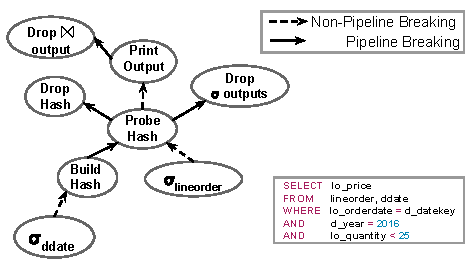
\includegraphics[width=\columnwidth]{policy/figures/QueryPlan.pdf}
	\vspace*{-2em}
	\caption{A join query and its DAG}
	\label{fig:dag}
%	\vspace*{-1.5em}
\end{figure}

The Query Manager uses a DAG Traversal algorithm (cf. Algorithm~\ref{alg:dag-traversal}) to process the DAG, which essentially is an iterative graph traversal method. 
The algorithm simply finds nodes in the DAG that have all their dependencies met, and marks such nodes as ``active'' (line~\ref{alg:depMet}).
Work orders are requested and scheduled for all active nodes (line~\ref{alg:getWork}), and 
the completion of work orders is monitored. 
Operators are stateful and they produce work orders when they have the necessary data.
The work order generation stops (line~\ref{alg:finishGenWork}) when the operators no longer have any input to produce additional work orders.
When no more work orders can be generated for a node, that node is marked as 
``completed'' (line~\ref{alg:nodeComplete}). 
When a node is marked as completed, all outgoing blocking edges (the solid lines 
in Figure~\ref{fig:dag}) are ``activated'' (line~\ref{alg:outEdgesActive}). 
Pipelining is achieved as all non-blocking edges (dotted lines in 
Figure~\ref{fig:dag}) are marked as active upfront (line~\ref{alg:pipelining}).
The query is deemed as completed when all nodes are marked as ``completed.''

% Note(harshad) - The DAG traversal example seems to be taking lots of space and can be omitted, as it diverts the attention away from the meat of the paper. 
%\subsubsection{DAG Traversal Example}\label{sssec:dag-traversal-example}
%To illustrate the execution of the scheduler algorithm, consider the 
%DAG shown in Figure~\ref{fig:dag}.
%Initially, only the two selection relational operators (shown in the DAG using
%the symbol $\sigma$) are \textit{schedulable}.\footnote{Initially, the print 
%operator is \textit{active} too, but as there's no input available, it can't
%produce any work order.}
%So, the Query Manager generates work orders for these operators. 
%In this case, there is one work order for each input block in each of the two
%input relations.\footnote{To avoid both select operators from being co-scheduled
%concurrently, a dependency link can be created between these two operators.
%Thus, work on the select operator on the $\mathtt{lineorder}$ table is started
%only after the select operator on the $\mathtt{ddate}$ table has completed. 
%Such decisions are made by the optimizer.}
%
%The Foreman assigns these work orders to the available worker threads. 
%The worker threads execute the operations specified in the work orders. 
%Note that given the independent block design (see Section~\ref{ssec:storage-manager}) 
%it is possible that two work orders on the same table may invoke different code paths. 
%For example one block on the \verb+ddate+ table may have an index sub-block on 
%the \verb+d_year+ attribute, and this index may be chosen to evaluate the tuples 
%in that block. 
%Another block on that same \verb+ddate+ table may not have any indices, and so 
%the selection operation for tuples in that second sub-block may resort to a simple scan. 
%In addition, the operator algorithm may choose to make a local decision on which 
%access plan to use. 
%So, e.g. even if each data block in the \verb+ddate+ table has an index 
%of the \verb+d_year+ attribute some work orders may use the index and others may 
%not. (The optimization algorithm for making these local decisions is beyond the 
%scope of this paper.)
%Essentially, the scheduler is largely oblivious to how the work orders are executed 
%and there is no global recipe that is imposed on the work orders that correspond 
%to a node in the DAG.
%
%Work orders may produce output data that are stored in blocks in the buffer pool. 
%In the case of the query in Figure~\ref{fig:dag}, the selection work orders on the \verb+ddate+
%table insert the selected tuples into data blocks that correspond to a new 
%temporary table. 
%%(the execution of the work orders is vectorized for efficiency). 
%These data blocks are pipelined to the next stage.\footnote{There is a 
%mechanism to allow multiple concurrent work orders from the same
%operator in the DAG to insert into a common output/temporary data
%block to avoid block internal fragmentation, and to facilitate early 
%pipelining. We omit these details.}
%In other words, as soon as there is a full block of tuples from applying the 
%selection operator on the \verb|ddate| table, a work order is created for the 
%\textit{build hash} operator. (Notice that the edge connecting the selection
%operator and the build hash operator permits data pipelining.)
%
%To begin the probe phase of the hash join, the building of the hash table must be 
%complete, as there is a pipeline-breaking dependency between the probe operator 
%and the build operator. 
%Thus, the DAG traversal algorithm only marks the probe hash operator node as 
%active when the build hash operator has completed. 
%Results from probing the hash table can be immediately pipelined to the print 
%operator.
%The drop operators ensure that intermediate data is dropped before the query is 
%deemed to have completed. 

\section{Resource Map Discussion}\label{apx:resource-map}
An example Resource Map of an incoming query to the system is shown below:
\begin{lstlisting}[language=python, 
								   basicstyle=\ttfamily\small, 
								   showstringspaces=false,
								   keywordstyle=\color{bondiblue}\bfseries, 
								   emph={CPU, Memory}, 
								   emphstyle=\color{cardinal}\bfseries]
CPU:    {min: 1 Core, max: 20 Cores}
Memory: {min: 20 MB,  max: 100 MB}
\end{lstlisting}

This Resource Map states that the query can use 1 to 20 cores (i.e. specifies the range of intra-operator parallelism) and is estimated to require a minimum of 20 MB of memory to run, and an estimated 100 MB of memory in the worst case.

In \sys{}, the query optimizer provides the estimated memory requirements for a given query.
Other methods can also be used, such as inferring the estimated resources from the previous runs of the query or other statistical analyses.
The scheduler is agnostic to how these estimates are calculated.

\section{Pipelining in \sys{}}\label{apx:pipelining}
During a work order (presumably belonging to a producer relational operator in a pipeline) execution, output data may be created (in blocks in the buffer pool). 
When an output data block is filled, the worker thread sends a ``block filled'' message to the corresponding query's manager via the following channel: Worker $\rightarrow$ Foreman $\rightarrow$ Policy Enforcer $\rightarrow$ Query Manager.
The Query Manager may then create a new work order (for a consumer relational operator in the pipeline) based on this information;
e.g. if this block should be pipelined to another operator in the query plan.

Note that pipelining in \sys{} works on a block-basis, instead of the traditional tuple-basis.

\section{Motivation for the Learning Agent Module}\label{apx:learning-motivation}
One might question the need of the Learning Agent and instead consider assigning a fixed probability value to each query (say $1/N$, with $N$ queries in the fair policy).
In the following section, we address this issue. 
A motivational example for the learning agent is described in Appendix~\ref{apx:learning-motivation}.

We perform an experiment, where the goal is to analyze the patterns in work order execution times of two queries. 
The dataset used for the experiment comes from the Star Schema Benchmark (SSB)~\cite{ssb} 
at a scale factor of 100. %(c.f. Section~\ref{ssec:workload} for benchmark details).
We pick two SSB queries $Q1.1$ and $Q4.1$, and execute them on a machine with 40 CPU cores. 
$Q1.1$ has a single join operation and $Q4.1$ has four join operations.
Figure~\ref{fig:q1.1-q4.1-time-per-wo} shows the observed average time per work order for both queries.
We now describe the trends in time per work order for the queries.

We can observe $Q1.1$'s execution pattern denoted by the dashed line in Figure~\ref{fig:q1.1-q4.1-time-per-wo}. 
The time per work order remains fairly stable (barring some intermittent fluctuations) from the beginning until 1.8 s.
This phase corresponds to the selection operation in $Q1.1$ which evaluates predicates on the \textit{lineorder} (fact) table.
A small bump in time per work order can be observed at the 1.8 s mark, when the probe phase of $Q1.1$ begins and continues until 2 s.
Towards the end of the execution of $Q1.1$, (2.2 s) there is a spike in time per work order when the query enters the aggregation phase. 
The output of the hash join is fed to the aggregation operation. 
The results of aggregation are stored in per-thread private hash tables, which are later merged to produce the final output.

\begin{figure}[h]
	\centering
	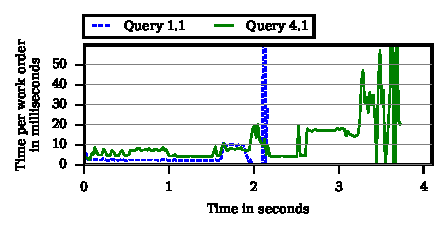
\includegraphics[width=\columnwidth]{policy/figures/q11-q41-time-per-wo.pdf}
	\vspace{-2.5em}
	\caption{Time per work order for Q1.1 and Q4.1}
	\label{fig:q1.1-q4.1-time-per-wo}
%	\vspace{-2em}
\end{figure}

Now we analyze the execution pattern for $Q4.1$ which has 4 join operations. 
This query is more complex than $Q1.1$.% which has a single join.
%Due to the more complex nature of the query, 
Therefore, the execution pattern of $Q4.1$ exhibits more phases, with different times per work order as compared to $Q1.1$.
Various small phases before the 0.5 s mark correspond to the selection predicates that are applied to the dimension tables. (Note that in $Q4.1$ there is no selection filter on the \textit{lineorder} table).
The selections on dimension tables get executed quickly.
The longer phases denote the different probe hash table operations in the query.
Towards the end, similar to $Q1.1$, there is a spike in the execution time per work order which correspond to the aggregation phase.

It is clear that the work order execution times for both queries are different, and the difference between them changes over time. 
If the scheduler assigns the same probability to both queries (i.e. 0.5), it is equally likely to schedule a work order from either of them. 
As a result, the queries will have different CPU utilization times in a given epoch, thus resulting in an unfair CPU allocation. 
In order to be consistently fair in allocating CPU resources to the queries, we should continuously observe the work order execution times of queries and adjust the CPU allocation accordingly. 

\section{Usage of Linear Regression in Learning Agent}\label{apx:linear-regression-usage}
The Learning Agent uses linear regression for predicting the execution time of the future work orders.
To lower the CPU and memory overhead of the model, we limit the amount of execution statistics stored in the Learning Agent.
We discard records beyond a certain time window. 
When all the work orders of an operator finish execution, we remove its records completely. 
In a query, if multiple relational operators are active, linear regression combines the statistics of all active operators and predicts a single value for the next work order execution time.

\section{Resource Choices for Policy Implementations and Load Controller Implementations}\label{apx:resource-discussion}
In the current implementation of \sys{}, we have focused on two key types of resource in the in-memory deployment scenarios -- CPU and memory. 
Both these resources have different resource characteristics, which we outline below.

First, consider the CPU resource. 
On modern commodity servers there are often tens of CPU cores per socket, and the aggregate number of cycles available per unit time (e.g. a millisecond) across all the cores is very large. 
Further, an implication of \sys{}'s fine-grained task allocation and execution paradigm is that the CPU resource can be easily shared at a fine time-granularity. 
Several work orders, each from different query can be executed concurrently on different CPU cores, and each query may execute thousands or millions or even more number of work orders. 
Thus, in practical terms, the CPU resource can be viewed as a nearly infinitely divisible resource across concurrent queries. 
In addition, overall system utilization is often measured in terms of the CPU utilization. Combining all these factors, specifying a policy  in terms of the CPU utilization is natural, and intuitive for a user to understand the policy. 
For example, saying that a fair policy equally distributes the CPU resource across all (admitted) concurrent queries is simple to understand and reason. 

Memory, on the other hand, is a resource that is allocated by queries in larger granular chunks. 
Active queries can have varying memory footprints (and the footprint for a query can change over the course of its execution). 
Thus, memory as a resource is more naturally viewed as a ``gating'' resource. 
Therefore, it is natural to use it in the load controller to determine if a query can be admitted based on its requested memory size. 
Actual memory consumption for queries can also be easily monitored, and when needed queries can be suspended if memory resource needs to be freed up (for some other query, perhaps with a higher priority). 

\section{Applicability of SSB for our evaluation}\label{apx:ssb}
The SSB is based on the TPC-H benchmark, and is designed to measure the query performance when %database systems in support of classical 
the data warehouse uses the popular Kimball~\cite{Kimball} approach. 
At a scale factor of X, the benchmark corresponds to about X GB of data in the 
corresponding TPC-H warehouse.
The SSB benchmark has 13 queries, divided in four categories. 
Each query is identified as \textbf{qX.Y}, where $X$ is the class and $Y$ is the query 
number within the class.
There are four query classes, i.e. $1\leq X\leq4$. 
The first and second classes have three queries each, the third class has four queries, and 
the fourth class has three queries.
The queries in each category are similar with respect to aspects such as the 
number of joins in the query, the relations being joined, the filter and aggregation 
attributes. 
The grouping of queries in various classes makes this benchmark suitable for our 
experiments, as it provides a way of assigning priorities to the queries based on their class. 

\section{Policy Enforcer}\label{apx:policy-enforcer}
The Policy Enforcer applies a high level policy for resource allocation among concurrent queries. 
It uses a probabilistic-framework to select work orders from a pool of work orders 
belonging to different concurrent queries for scheduling. 
The Policy Enforcer assigns a probability to each active query, which indicates the likelihood of a work order from that query getting scheduled for execution in the near future. 
The probability-based work order selection strategy brings powerful control to the scheduler through a single parameter -- i.e. by controlling the probability 
setting, the scheduler can control the resource sharing among concurrent queries. 
%A work order from a query with higher probability is more likely to get scheduled 
%than a work order from a query with lower probability. 

The challenge in designing the policy enforcer lies in transforming the policy specifications to a set of probabilities. 
A critical piece that we use in such transformations is the prediction of work order 
execution times for the concurrent queries, which is done by the Learning Agent. 
%described in Section~\ref{ssec:learning}. %and depicted in Figure~\ref{fig:scheduler-cycle}.
In the remainder of this section, we provide an intuition for deriving probability values from the work order execution times. 
%A formal model for the probability computations for different policies is presented in Section~\ref{sec:policy}.

\begin{figure}[]
	\centering
	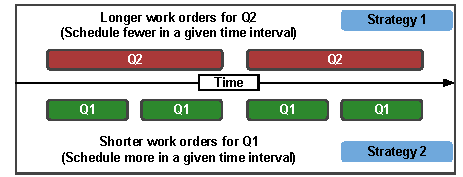
\includegraphics[width=\columnwidth]{policy/figures/Probability-explanation.pdf}
	\vspace{-2em}
	\caption{Scheduling queries having different work order execution times for the fair policy. The solid boxes with $Q_{i}$ depicts the lifetime of a work order from the Query $Q_{i}$.}
	\label{fig:probability-explanation}
	%	\vspace{-1.5em}
\end{figure}

We now motivate the probabilistic approach used by the Policy Enforcer with an example.
Consider a single CPU core and two concurrent queries $q_{1}$ and $q_{2}$. 
(The idea can be extended to multi-cores and more than two queries.)
Initially, we assume perfect knowledge of the execution times of work orders of the queries. 
Later, we will relax this assumption. 

Let us assume that as per the policy specifications, in a given time interval, the CPU resources should be shared equally. 
Suppose that work orders for $q_{1}$ take less time to execute than work orders for 
$q_{2}$, as shown in Figure~\ref{fig:probability-explanation}.
As the Policy Enforcer aims to allocate equal share of the CPU to $q_1$ and $q_2$, a simple strategy can be to schedule proportionally more work orders of $q_{1}$  than those of $q_{2}$, in a given time window. 
The number of scheduled work orders is inversely related to the work order execution 
time. 
This proportion can be determined by the probabilities $pb_{1}$ and $pb_{2}$ for queries $q_1$ and $q_2$, respectively.
The probability $pb_i$ is the likelihood of the scheduler scheduling next work order from query $i$. 
The probability is assigned by the Policy Enforcer to each active query in the system.
Note that, $pb_{1} > pb_{2}$ and $pb_{1} + pb_{2} = 1$.

%Such strategy will result in similar \textit{CPU occupancy} with respect to time 
%for both the queries, thereby fairly sharing the CPU resource in a given time 
%frame.  If the policy enforcer keeps scheduling the work orders similarly for the rest of 
%the  workload execution, it is easy to see that the queries will share the CPU 
%\textit{fairly}, as demanded by the policy. 

Notice that the Policy Enforcer is not concerned with the complexities of the operators in the query DAGs. 
It simply maintains the probability associated with each active query which is determined by the query's predicted work order execution times.

The Policy Enforcer can also function with workloads that consist of queries categorized in multiple classes, where each class has a different level of ``importance'' or ``priority''. 
The policy specifies that the resource allocation to a query class must simply be in accordance to its importance, i.e. queries in a more important class should collectively get a higher share of the resources, and vice versa.
In such scenarios, the Policy Enforcer splits its work order selection strategy in two steps - selection of a query class and subsequent selection of a 
query within the chosen query class.
Intuitively, the Policy Enforcer should assign higher probability to the more 
important class and lower probability to the less important class.

Once a query class is chosen, the Policy Enforcer must pick a query from the chosen class. 
Each query class can specify an optional intra-class resource allocation sub-policy. 
By default, all queries within a class are treated equally.
Thus, the probability-based paradigm can be used to control both inter and intra-class resource allocations.

There could be many reasons for categorizing queries in classes, including the need to associate some form of urgency (e.g. interactive vs batch queries), or marking the importance of the query source 
(e.g. the position of the query submitter in an organizational hierarchy). 
In addition, the resource allocations across different classes can also be chosen based on various scales, such as linear or exponential scale allocations based on the class number. 
An attractive feature of the Policy Enforcer is that it can be easily configured for use in a variety of ways.
Under the covers, the Policy Enforcer simply maps each class to a collective class probability value, and then maps each query in each class to another probability. 
Once these probabilities are calculated, the remaining mechanisms simply use them to appropriately allocate resources to achieve the desired policy goal.
		%% Add sample pairs etc. 0.5 day
%\end{appendix}

%=======================================================================
% Index
%\begin{singlespace}
%\printindex
%\end{singlespace}

%\include{vita}                  % Optional Vita, use \begin{vita} vita text \end{vita}
\end{document}
